\documentclass[
 reprint,
 amsmath,amssymb,
 aps,
]{revtex4-2}
\usepackage[spanish]{babel} % This sets the main language of the document to Spanish.lign table columns on decimal point
\usepackage{graphicx}
\usepackage{bm} % bold math
\usepackage{float}
\usepackage{listings}
\usepackage{color}
\definecolor{codebg}{gray}{0.96}
\definecolor{coderule}{gray}{0.6}
\definecolor{codegray}{gray}{0.3} 
\lstset{ 
  language=c++,
  backgroundcolor=\color{codebg},
  basicstyle=\ttfamily\footnotesize,       % Fuente base
  commentstyle=\itshape\color{codegray},
  stringstyle=\ttfamily,
  numberstyle=\tiny\color{codegray},
  numbers=left,
  numbersep=10pt,
  frame=single,
  frameround=tttt,
  rulecolor=\color{coderule},
  breaklines=true,
  breakatwhitespace=true,
  showstringspaces=false,
  captionpos=b,
  tabsize=4,
  emphstyle=\bfseries
} 
\begin{document}
\preprint{APS/123-QED}

\title{Determinación de la carga elemental\\ mediante un análisis del experimento de Millikan} 

\author{Angel Eduardo Luna Leija}  
\author{Salvador Alejandro Martin Garza}
\author{Axel Dair Peña Cruz}
\author{Jazmin Padilla Ramos}
\affiliation{
  Instituto Tecnológico y de Estudios Superiores de Monterrey - Campus Monterrey
}
\date{\today} % Fecha en formato español

\begin{abstract}
    El presente informe tiene como finalidad introducir el objetivo general del proyecto: la determinación de la carga elemental del electrón mediante la simulación computacional del experimento de Millikan. Para ello, se proporciona un marco teórico que permite comprender los fundamentos físicos del experimento, así como los parámetros que influyen en su desarrollo. Esta base teórica se construyó a partir de una revisión bibliográfica sustentada en artículos científicos especializados.

    La simulación del experimento fue implementada en el lenguaje de programación C++, utilizando las expresiones matemáticas pertinentes, tales como la ley de Stokes, la corrección de Cunningham y la ecuación del campo eléctrico. Tras realizar múltiples pruebas variando los parámetros del sistema, se obtuvo una estimación aproximada de la carga del electrón, lo cual valida la precisión teórica del método propuesto y demuestra la viabilidad de su implementación computacional.
\end{abstract}

\maketitle 

\section{\label{sec:level1}Introducción} 
El desarrollo de este proyecto colaborativo consiste en elaborar una simulación numérica del experimento de la gota de aceite de Millikan, el cual fue realizado por Robert Millikan y su estudiante Harvey Fletcher en 1909 \cite{reto}. Este experimento tuvo un gran impacto ya que logró medir con precisión la carga elemental del electrón, lo cual ayudó al desarrollo de varios campos, como la electrónica, la física cuántica y la nanotecnología.

Durante este proyecto, se construirá una simulación numérica del experimento de Millikan, considerando factores físicos para modelar el comportamiento de gotas de aceite cargadas en un campo eléctrico. Se deberá hacer un análisis de los datos obtenidos, así como una explicación de los fundamentos físicos y las ecuaciones y algoritmos utilizados. Finalmente, se obtendrá el valor de la carga elemental del electrón con una precisión superior al 90\% con respecto al valor aceptado actualmente.

Entonces, tomando en consideración el objetivo y procedimiento que se llevará a cabo durante este proyecto, antes de iniciar el reto necesitamos conocimientos previos como los conceptos de carga, campo eléctrico y ecuaciones básicas de dinámica para comprender el movimiento de las gotas y su significado. También necesitamos entender cómo se llevó a cabo el experimento de Millikan, y qué conceptos y ecuaciones influyeron en él. Por otro lado, durante la elaboración del proyecto desarrollaremos habilidades como el cálculo de fuerzas en un campo eléctrico, cálculo de intensidad de un campo eléctrico, relaciones entre voltajes, entre otros. También se desarrollarán habilidades para desarrollar el modelo computacional para simular cada componente del sistema y representarlo de manera gráfica. 

\section{\label{sec:level2}Experimento de Millikan}

\subsection{\label{sec:citeref}Configuración experimental}

El experimento trata sobre dejar un conjunto de gotas cargadas eléctricamente caer entre las dos placas de metal horizontales conectadas a una fuente de potencial eléctrico variable. Primeramente, sin establecer alguna diferencia de potencial entre ellas, las gotas caen a una velocidad terminal calculada asumiendo una fricción viscosa de Stokes, hasta que la fuerza friccional es igual a su peso. Al momento de que un voltaje es aplicado, aparece una fuerza eléctrica, que la levanta a su altura original. Y sea cual sea la fricción, la carga eléctrica es proporcional  a la suma de las velocidades.
En general, el experimento comienza produciendo una nube de gotas que caen por un pequeño hueco en la placa superior. Son cargadas eléctricamente ya sea por la fricción o por la exposición a los rayos X o la luz ultravioleta. Después, son observadas con un microscopio, que se concentra en su trayectoria y se mide el tiempo en el que tardan en caer. Al activar el campo eléctrico, se mide el tiempo que toma para subir de nuevo. Así, se realizan los diversos cálculos sobre las varias gotas analizadas por el experimento. En la cual se pueden obtener los valores aproximados a $\text{e}_c=4.803\times 10^{-10}$.\cite{hector2020}

\begin{figure}[H]
    \centering
    \includegraphics[width=0.7\linewidth]{Scheme_of_Millikan’s_oil-drop_apparatus.png}
    \caption{Gráfico de la configuración del aparato usado para la realización del experimento de Millikan.\cite{millikan1913}}
    \label{fig:aparato}
\end{figure}


\subsection{\label{sec:citeref}El porqué}
Desde que se dio a conocer la existencia de la partícula del electrón y su masa por parte de J.J. Thompson, fue una alta prioridad por parte de los científicos de la época descubrir la carga eléctrica que esta partícula posee, es por esto que R.A. Millikan diseñó su reconocido experimento; se debe considerar también que esto fue un proceso de varios años. Ya que los resultados inicialmente fueron lamentables, Millikan pasó gran parte de su tiempo refinando partes de este experimento para obtener resultados óptimos.\cite{hector2020}



\subsection{\label{sec:citeref}Fuerzas físicas sobre las gotas de aceite}
Para entender cómo funcionó el experimento, primero se debe entender cuáles son las fuerzas físicas que afectan a las gotas de aceite. El experimento requiere la fuerza gravitacional de Newton, dada por la ecuación:
\begin{equation}
F_g = m \cdot g
\label{eq:Fg}
\end{equation}

Esto se debe a que las gotas de aceite son afectadas por la gravedad del planeta.

La ley de Stokes también juega un papel importante en el experimento, ya que se debe calcular el radio de la gota de aceite. Estas gotas terminan siendo cuerpos esféricos que caen en un medio viscoso con una velocidad terminal. Según la ley de Stokes, la fuerza está dada por:
\begin{equation}
F = 6 \pi r \eta v
\label{eq:Fv}
\end{equation}

donde \(\eta\) es la viscosidad del fluido (aire) en el cual caen las gotas de aceite, \(r\) es el radio de las gotas, y \(v\) es la velocidad.

Dado que la densidad del aire es menor que la densidad del aceite, no se incluirá el principio de Arquímedes \cite{RSEF2011}.

La última fuerza que actúa sobre las gotas es la fuerza eléctrica, definida como:
\begin{equation}
F_e=qE
\label{eq:Fe}
\end{equation}

Esto se debe a que se genera un campo eléctrico. En la fórmula, \(q\) representa la carga neta de la gota, y \(E\) es la intensidad del campo eléctrico entre las placas \cite{Luna_sf}\cite{UofToronto_sf}.

\subsection{\label{sec:citeref}Principios de electrostática relevantes para el experimento}
Los principales fundamentos de la electrostática aplicados en este experimento fueron, en general:
\begin{itemize}
  \item Así como las fuerzas de cargas similares se repelen, las fuerzas de cargas diferentes se atraen.
  \item Esta línea o vector de repulsión o atracción actúa en la línea entre estas dos fuerzas, es decir, la distancia.
\end{itemize}
Estos principios se basan en la ley establecida por Coulomb, que explica:
\begin{center}
\textit{``The magnitude, or absolute value, of the attractive or repulsive electrostatic force between two point charges is directly proportional to the product of the magnitudes of their charges and inversely proportional to the square of the distance between them''.}\cite{Coulomb1785}
\end{center}
Lo cual se ve de la siguiente manera:
\begin{equation}
F(r)=\frac{q}{4\pi\varepsilon_0}\sum_{i=1}^nq_i\frac{\hat{r}_i}{|r_i|^2}
\label{Coulomb}
\end{equation}

\subsection{\label{sec:levels}Ley de Stokes}
Esta ley relaciona las características de fricción de un fluido con fuerzas externas, como la gravedad, inercia y fuerzas electromagnéticas. 
La fórmula se expresa como: el peso de la partícula es igual al empuje de Arquímedes más la fuerza de fricción. Se representa de la siguiente forma:
\begin{equation}
   \frac{4}{3}\rho_p\pi R^3g=\frac{4}{3}\rho f\pi R^3g+6\pi R\eta V 
   \label{stokes}
\end{equation}
Donde:
\begin{itemize}
  \item R = radio de la partícula
  \item \(\rho_p\) = densidad de la partícula
  \item \(\rho\)f = densidad del fluido
  \item \(\eta\) = viscosidad del fluido
  \item g = fuerza de la gravedad
  \item V = velocidad terminal de sedimentación
\end{itemize}
Por lo que, si se requiere despejar la velocidad, la fórmula queda como:
\begin{equation}
    V=\frac{2(\rho_p-pf)gR^2}{g\eta}
\end{equation}

Como se puede ver, la velocidad de sedimentación es proporcional a la diferencias de densidades de los materiales, a la gravedad y al cuadrado del radio de la partícula, e inversamente proporcional a la viscosidad del líquido.
Es importante mencionar que la ley funciona en sistemas en donde las partículas son esferas sin deformaciones, y se mueven de manera suave y sin turbulencias.
Un ejemplo práctico de esta ley es la caída de gotas de lluvia en el aire o la sedimentación de partículas en líquidos, como en la purificación de agua o la formación de capas en mezclas heterogéneas \cite{shearer2008fluid}.
La ley de Stokes tiene una relación directa con el experimento de Millikan, ya que ambos estudian el movimiento de partículas esféricas a través de un fluido. En el experimento de Millikan, pequeñas gotas de aceite cargadas eléctricamente caían a través del aire dentro de una cámara controlada. Durante su caída, estas gotas alcanzaron una velocidad terminal debido a la resistencia del aire, la cual puede describirse mediante esta misma ley.


\subsection{\label{sec:levels}Escenarios sin campos eléctricos y con campos magnéticos}

Al no existir un campo eléctrico presente en el experimento, se podría reemplazar con uno magnético que termine aplicando una fuerza neta igual que logre llegar a un equilibrio en el experimento. Según un experimento realizado por la universidad de Nuevo México, el cual sirve muy bien como analogía para el experimento de Millikan tomando en cuenta las condiciones anteriores planteadas. Por lo que, experimentalmente, se puede realizar con resultados prácticos y aptos que se asemejan bastante al experimento original.
La relación entre electricidad y magnetismo viene dada por las ecuaciones de Maxwell que las integran como un solo principio físico. La ecuación es la siguiente:

\begin{equation}
    F=q(E+B\times v)    
\end{equation}

Donde:
\begin{itemize}
    \item $F$ es la fuerza total sobre una partícula con carga q.
    \item $E$ es el campo eléctrico $(V/m)$.
    \item $B$ es el campo magnético $(T)$.
    \item $v$ es la velocidad de la partícula $(m/s)$.
    \item $\times$ representa el producto cruzado, lo que significa que la fuerza magnética es perpendicular a la dirección del movimiento de la carga.\cite{pearson1313}
\end{itemize}

\subsection{\label{sec:levels}Ecuaciones de equilibrio}

En la realización del experimento  las gotas de aceite alcanzaron un estado de equilibrio en el que la suma de la fuerza viscosa y la fuerza de gravedad es de igual magnitud pero en sentido opuesto al campo eléctrico, por lo que su fuerza total es nula, su aceleración es 0 y su velocidad es constante \cite{Mera_Ayala_2015}. Esto fue de vital importancia para la realización del experimento y para la obtención de resultados sobre la carga del electrón. El balance de fuerzas se ve de la siguiente manera:

\begin{figure}[H]
    \centering
    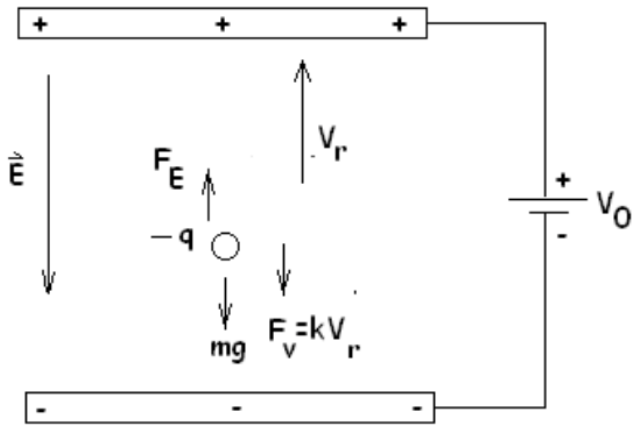
\includegraphics[width=0.7\linewidth]{Screenshot 2025-04-02 at 15.10.25.png}
    \caption{Gráfico que ilustra el balance de fuerzas en situación de subida recuperado de Mera y Ayala \cite{Mera_Ayala_2015}}.
    \label{fig:balance}
\end{figure}
\begin{equation}
    F_e=F_g+F_v
\end{equation}
\begin{equation}
    qE=mg+6 \pi r \eta v
\end{equation}

Recordando que:
\begin{itemize}
    \item La fuerza elétrica se define en la ecuación \ref{eq:Fe}.
    \item La fuerza de gravedad se define en la ecuación \ref{eq:Fg}.
    \item La fuerza viscosa se define en la ecuación \ref{eq:Fv}.
\end{itemize}

\subsection{\label{sec:levels}Parámetros físicos clave}
Los siguientes son parámetros físicos identificados por tener alta relevancia en la realización del experimento:
\begin{itemize}
    \item La forma de la gota ya que se asume que es esférica por lo que se usará la ley de Stokes.
    \item El radio de la gota ya que va a influir en la fuerza de arrastre y en la velocidad terminal.
    \item La densidad de la gota de aceite determina su masa y la fuerza de gravedad que actúa sobre ella.
    \item La masa de la gota de aceite la cual se obtiene de la siguiente fórmula: 
    \begin{equation}
        \frac{4}{3}\pi R^3P
    \end{equation}
    \item La carga neta de la gota ya que se requiere saber la cantidad de carga eléctrica adquirida. 
    \item La temperatura se requiere considerar porque afectará la viscosidad del aire y el movimiento de la gota.
    \item El campo eléctrico influye en la fuerza aplicada sobre la gota, explicado en la ecuación \ref{eq:Fe}.
    \item El voltaje aplicado también es un factor ya que controla la intensidad del campo eléctrico.
    \item Las distancias entre las placas influyen en los cálculos del campo eléctrico.
    \item La aceleración de gravedad que actúa sobre la gota.
    \item La fuerza de arrastre que se obtiene a través de la ley de stoke descrita en la ecuación \ref{eq:Fv}.
    \item El tiempo de caída se debe considerar ya que se debe determinar la velocidad con la que cae la gota.
    \item La velocidad terminal se considera para determinar cuando la gota alcanza un equilibrio de fuerzas \cite{UofToronto_sf}\cite{RSEF2011}.
\end{itemize}

\section{\label{sec:levels}La simulación}

Despu\'es de haberse establecido los fundamentos te\'oricos y la informaci\'on necesaria para entender a detalle el experimento de la gota de aceite de Millikan, se requiere comprobar si la simulaci\'on del movimiento de las gotas influenciadas por las placas se puede replicar computacionalmente y lograr los resultados esperados de la realizaci\'on del experimento de manera f\'isica. Esto demostrar\'ia que la capacidad de la modelaci\'on computacional de los fen\'omenos involucrados en el experimento son realizables.

\subsection{Definici\'on de f\'ormulas}

Definiremos las fórmulas utilizando la información recabada anteriormente, por lo cual se incluyen las referencias que se utilizaron en ese reporte en el apartado de referencias.

Para definir la la velocidad terminal (VF)  en caída libre sin el campo eléctrico que alcanza la gota se deben restar las fuerzas. La fuerza de peso de la gota se contrarresta contra la fuerza de flotación y la resistencia del aire. 

\begin{equation}
    F_W-F_A-F_D=0
\end{equation}
\begin{itemize}
    \item Fuerza de gravedad (peso):
    \begin{equation}
    F_W=mg=\frac{4}{4}\pi r^3\rho_\text{oil}g
    \end{equation}

    \item Fuerza de flotaci\'on:
    \begin{equation}
    F_A=\frac{4}{3}\pi r^3\rho_\text{aire}g
    \end{equation}

    \item Resistencia de viscosidad (ley de Stokes):
    \begin{equation}
    F_D = 6 \pi \eta r v
    \end{equation}

    \item Correcci\'on de Cunningham para gotas peque\~nas:
    \begin{equation}
    F_D = \frac{6 \pi \eta r v}{1 + (b/(p r'))}
    \end{equation}

    \item Radio de la gota:
    \begin{equation}
    r = \sqrt{\frac{9 \eta v}{2 g (\rho_{\text{aceite}} - \rho_{\text{aire}})}}
    \end{equation}

    \item Campo el\'ectrico entre placas:
    \begin{equation}
    E = \frac{V}{d}
    \end{equation}

    \item Carga cuando la gota asciende:
    \begin{equation}
    q = \frac{6 \pi \eta r (v_{\text{ascenso}} + v_{\text{ca\'ida}})}{E (1 + b/(p r'))}
    \end{equation}

    \item Carga en equilibrio:
    \begin{equation}
    q = \frac{(m g - F_b) d}{V}
    \end{equation}
\end{itemize}

El conocimiento del radio, la velocidad de ca\'ida y ascenso, el campo el\'ectrico aplicado, junto con las constantes f\'isicas del aceite, aire y viscosidad, permite calcular de manera precisa la carga elemental en las gotas de aceite.

\subsection{Desarrollo computacional}

Se utiliz\'o C++ como lenguaje de programaci\'on para modelar toda la simulaci\'on del experimento. Los valores iniciales fueron:

\begin{itemize}
    \item Densidad del aceite: 919.9 $kg/m^3$
    \item Gravedad: 9.803 $m/s^2$
    \item Densidad del aire: 1.2 $kg/m^3$
    \item Viscosidad del aire: $1.81\times10^{-5} kg/ms$
    \item Distancia entre placas: $16\times10^{-3}m$
    \item Voltaje entre placas: 5 $kV$
    \item Presi\'on: 13438.7 $Pa$
    \item Radio de la gota: aleatorio entre 2.780 y 2.790 $\mu m$
    \item Carga de la gota: aleatorio, m\'ultiplo de la carga del electr\'on
\end{itemize}

Estos parámetros están basados en el experimento de la gota “6” realizado por Millikan \cite{Millikan1912} \cite{Oxford}. El radio y la carga de la gota los decidimos de manera aleatoria porque eran valores que Millikan no conocía al momento de hacer su experimento, así mantenemos la naturaleza del experimento de descubrir la carga aunque se trate de una simulación.

Con una delta de tiempo de 1x10$^{-6}$ y utilizando las ecuaciones ya mencionadas ciclamos el cambio de aceleración, velocidad y posición de las gotas hasta que el valor absoluto de su aceleración fuese menor a 1x10-5 m/s2, es decir, cuando la velocidad es casi constante. Simulamos una trayectoria sin y con campo eléctrico, esto quiere decir que en la trayectoria con campo se agregó a la suma de las fuerzas la fuerza que experimentaría la gota por el campo eléctrico, lo cual es vital para hacer la comparación de velocidades finales y obtener la carga de la gota. 

También agregamos que los datos se vayan guardando en un documento .csv, el cual utilizamos para graficar la velocidad de cada gota por separado, utilizando Python.


\begin{figure}[H]
\begin{lstlisting}
    while (abs(gotas[i].indexacc(j))>1e-6 or gotas[i].indexacc(j)==0)
    {
        double drag=-6*M_PI*airV*gotas[i].getrad()*
            gotas[i].indexvelociry(j)/(1+(b/
                pressure*gotas[i].getrad()));
        gotas[i].defdrag(drag);
        double acceleration=(gotas[i].getweight()+
            drag+gotas[i].getbuoyant())/
                gotas[i].getmass();
        gotas[i].Acc(acceleration);
        double vel= gotas[i].indexvelociry(j)+
            gotas[i].indexacc(j)*deltaT;
        gotas[i].Vel(vel);
        double height=gotas[i].indexheight(j)-
            vel*deltaT;
        gotas[i].p_height(height);
        gotas[i].p_time(gotas[i].indextime(j)+
            deltaT);
        
        j++;
    }
\end{lstlisting}
\caption{Ciclo para la trayectoria sin campo el\'ectrico.}
\end{figure}

\subsection{Resultados}

Se simularon cinco gotas bajo par\'ametros distintos. Los resultados se muestran a continuación:

\begin{table}[H]
\centering
\resizebox{\columnwidth}{!}{
\begin{tabular}{c c c c}
\hline
Gota & Velocidad con campo (m/s) & Velocidad sin campo (m/s) & Carga de la gota (C) \\
\hline
\hline
0 & 0.000359912 & 0.000640526 & 2.5086e-18 \\
1 & 9.64279e-05 & 0.000640065 & 1.84598e-18 \\
2 & 0.00062949 & 0.000643293 & 3.19959e-18 \\
3 & 0.000630423 & 0.000644216 & 8.13459e-19 \\
4 & -0.000378018 & 0.000640065 & 6.56807e-19 \\
\hline
\hline
\end{tabular}
}
\caption{Valores de velocidad y carga para cada gota simulada.}
\end{table}

\begin{figure}[H]
\centering
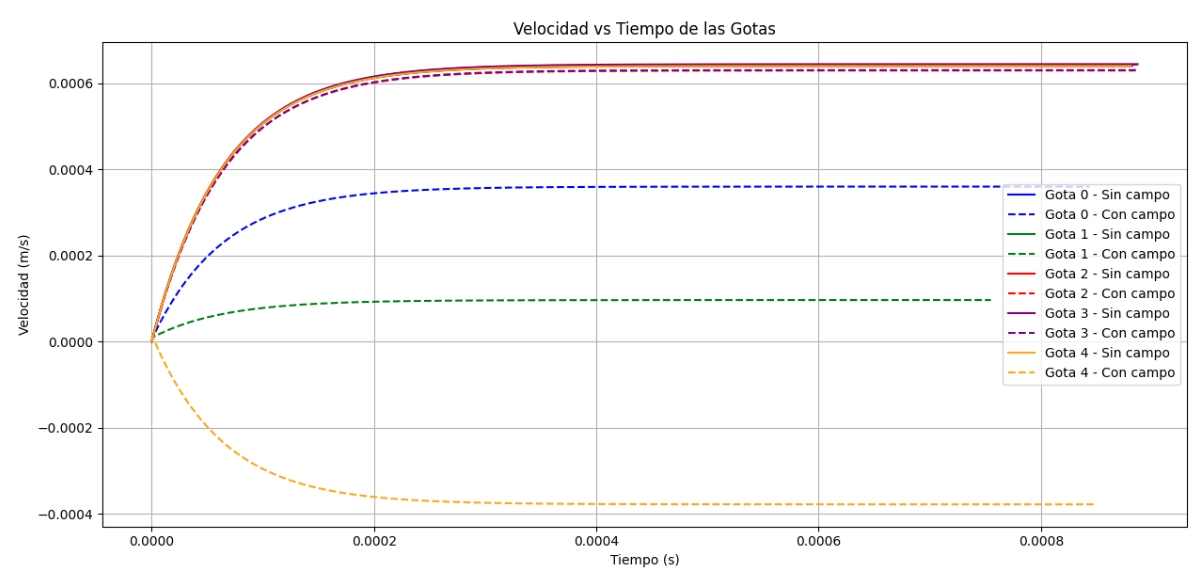
\includegraphics[width=0.48\textwidth]{Screenshot 2025-04-27 at 22.22.51.jpg}
\caption{Gr\'afica de velocidad vs. tiempo para las gotas simuladas.}
\end{figure}

\section{An\'alisis de resultados}

Como se esperaba, la velocidad de la gota fue cambiando hasta alcanzar una velocidad terminal casi constante, estas velocidades terminales son muy similares, lo cual indica que las condiciones iniciales fueron consistentes. Al activar el campo eléctrico, las velocidades de las gotas se alteran significativamente, algunas aumentan o disminuyen, lo que refleja correctamente el funcionamiento del campo sobre diferentes cargas. 

Al comparar nuestros resultados con los reportados por Millikan, podemos encontrar que tanto la velocidad, como la carga de las gotas es muy similar a lo que él experimentó, por lo que la simulación es fiel al fenómeno real. No tiene caso buscar deducir la carga del electrón a partir de estos resultados porque esta ya se tomó en cuenta en los parámetros, sin conocerla, no se hubiera podido realizar la simulación. Sin embargo, realizar esta simulación ha sido un ejercicio enriquecedor para el entendimiento del comportamiento de las cargas y el reconocimiento de la importancia de la carga del electrón como la carga elemental, la cual es -1.602x10$^{-19}$ coulombs.

\section{Conclusi\'on}
La simulación del experimento de Millikan sí se pudo replicar de manera teórica gracias a los fenómenos físicos que se descubrieron años atrás. Por medio de la implementación de modelos de fuerzas y otros parámetros que se representan lo mejor posible, como la gravedad, fuerza de flotación, de arrastre y eléctrica, fue posible obtener valores congruentes con los medidos en el experimento original. Todo esto demuestra que es importante tomar en cuenta todas las variables posibles si se quiere modelar un sistema físico, y mientras más precisión se requiera a la hora de simular tales fenómenos, se requeriría de una mayor comprensión de las fuerzas físicas.

% The \nocite command causes all entries in a bibliography to be printed out
% whether or not they are actually referenced in the text. This is appropriate
% for the sample file to show the different styles of references, but authors
% most likely will not want to use it.
\nocite{*}

\bibliography{bibliography}% Produces the bibliography via BibTeX.

\end{document}
%
